\chapter{Úvod}
\label{cha:introduction}

Steganografie je obor zabývající se skrýváním informace takovým způsobem, aby
nebylo možné zjistit její přítomnost. Důvod pro takovéto skrývání informace
může být zajištění bezpečnosti před nějakou třetí stranou pro kterou není
informace určena. Steganografie se dnes dělí na tradiční a~digitální.
V~digitální steganografii je velké množství typů dat do kterých je možné vkládat
utajované informace a~digitální zvuk je jedním z~nich.

V~oblasti digitální zvukové steganografie je dostupné velké množství kvalitní
literatury popisující teoretické fungování metod, kterými se jednotlivé
publikace zabývají. Je však těžké najít konkrétní implementace popisovaných
metod i~přesto, že autoři je implementovali pro získání výsledků. Proto je
hlavním cílem této práce vytvořit softwarovou knihovnu a~program
v~programovacím jazyce Python, aby měl kdokoliv možnost pracovat na výzkumu
v~této vědecké disciplíně. Někdy totiž nestačí pouze algoritmický popis různých
metod pro pochopení jejich fungování. Implementace v~konkrétním programovacím
jazyce nám přináší formalismus, který umožňuje snazší pochopení. Chtěl bych
proto touto prací přispět v~této oblasti tím, že bude přístupnější pro širší
veřejnost.

V~následujících kapitolách této práce je shrnut současný stav tohoto oboru,
jsou vysvětleny cíle a~technické prostředky použité k~jejich dosažení
a~zhodnoceny dosažené výsledky. V~kapitole~\ref{cha:existing-methods}
\uv{Význam steganografie a~přehled existujících metod digitální zvukové
steganografie} jsou do hloubky popsány steganografické metody vybrané pro
implementaci a~některé další používané. Kapitola~\ref{cha:library-design}
popisuje proč byl vybrán programovací jazyk Python a~použité knihovny. Je zde
také popsána struktura balíčků pro Python a~steganografické metody které byly
vybrány pro implementaci včetně vlastní. Kapitola~\ref{cha:implementation} je
zaměřená na popis rozvržení kódu a~implementaci steganografických metod. Na
konci kapitoly je popsán způsob vyhodnocení kvality metod, výsledky testování
a~srovnání metod. Na závěr kapitola~\ref{cha:conclusion} obsahuje shrnutí
výsledků práce a~vyhlídky do budoucna.


\chapter{Význam steganografie a~přehled existujících metod digitální zvukové
steganografie}
\label{cha:existing-methods}

Tato kapitola představí širší možnosti využití steganografie v~dnešním světě.
Poté bude stručně popsán způsob jakým se dnes reprezentuje digitální zvuk. Dále
budou vysvětleny vlastnosti na základě kterých budou metody hodnoceny
a~srovnávány. Každá z~podkapitol která bude následovat, se zaměří na některou
z~používaných steganografických metod a~jejich možné modifikace.

\section{Význam steganografie a~její využití}
\label{sec:motivation-and-uses}

Steganografie je praktika skrývání informace s~cílem zakrýt její samotnou
existenci a~ne jen znemožnit její čtení
\cite{AlSabhany2020}\cite{Anderson1998}\cite{Djebbar2012}\cite{Dutta2020}.
Původ této praktiky se vrací až do antiky -- vyrytím písma do destičky, která
se následně zalila voskem; ve středověké Evropě položením papíru nebo dřevěné
šablony na nevinně vypadající text, čímž zvýrazní tajnou zprávu. Steganografie
se tedy v~různých podobách praktikovala po tisíciletí až do dnešní počítačové
doby \cite{Anderson1998}, kdy je považována za podobor zabezpečení dat
\cite{Djebbar2012} a~více se přesouvá od tradiční k~digitální steganografii.

V~dnešním světě se stalo zabezpečení dat zájmem všech a~steganografie jako
proces ukrývání zprávy do jiného typu média slouží k~ochraně před
neautorizovanými či neoprávněnými příjemci \cite{Dutta2020}. Médium do kterého
je informace skrývána se nazývá nosič a~může být různých typů, jako například
obrázek, audio, video, IP datagram \cite{Dutta2020}, text a~mnoho dalších.
Každý typ nosiče má svoji oblast výzkumu, která se jej týká. Některé
steganografické metody používané u~různých typů nosičů jsou konceptuálně stejné
a~v~praxi se aplikují podobným způsobem. Tato práce se však bude zabývat pouze
metodami použitelnými pro digitální audio.

Poslední dobou se začaly objevovat nové směry založené na steganografických
přístupech pro zajištění bezpečnosti a~utajení dat které by v~kombinaci
s~konvenčními bezpečnostními technikami mohly vést k~lepším výsledkům
\cite{Djebbar2012}. Jedna z~konvenčních bezpečnostních technik kombinovaných se
steganografií je kryptografie. Zatím co steganografie se zabývá ukrýváním
informace, hlavním cílem kryptografie je převést zprávu do formy, která je pro
neoprávněné osoby nečitelná \cite{AlSabhany2020}. I~když se tedy někdo pokusí
analyzovat komunikaci pro přítomnost utajené zprávy, není možné obsah rozeznat
od náhodného šumu.

Steganografie má široké spektrum využití. Mezi praktické příklady patří:
monitorování reklam v~rádiu, indexování video zpráv, použití všude tam, kde
není možné použít šifrování, zachování soukromí jednotlivce, utajená komunikace
mezi vojenskou rozvědkou nebo bezpečnostními složkami~\cite{Dutta2020}.

Dalším často používaným pojmem spojeným se steganografií je vodoznak. Vodoznaky
se používají pro vložení informací o~původu, vlastnictví, či autorských právech
dat \cite{Djebbar2012}\cite{Dutta2020}\cite{Swanson1998}. Hlavní vlastností
vodoznaku je, že by nemělo být možné jej odstranit bez poškození nosného média.
Proto u~audia nesmí být součástí hlavičky souboru nebo být přenášen zvlášť, ale
být jeho součástí a~musí být nedetekovatelný. Musí být také odolný proti
transformaci signálu například při přenosu audia nebo převedení do formátu,
který používá ztrátovou kompresi \cite{Swanson1998}. Velice známým příkladem
jsou vodoznaky na bankovkách nebo \textit{žluté tečky} v~tiskárnové
steganografii -- známé také jako \textit{yellow dots} -- které barevné tiskárny
tisknou na každý list. Tyto tečky obsahují zakódované sériové číslo tiskárny
a~čas tisku \cite{Dutta2020}. Pokud je vodoznak použit pro ochranu
intelektuálního vlastnictví, pak se ještě rozlišuje mezi vodoznakem a~otiskem.
Vodoznakem se značí všechny objekty stejně, ale otisk se může měnit například
pro každého zákazníka pro jeho pozdější identifikaci. To může být užitečné
pokud poruší licenční podmínky například sdílením zakoupené hudby
\cite{Swanson1998}.

\section{Reprezentace a~způsob uložení digitálního zvuku}
\label{sec:digital-sound-representation}

\todo{popis způsobu uložení digitálního zvuku}

\blindtext

\blindtext

\section{Vlastnosti metod digitální zvukové steganografie}
\label{sec:method-properties}

\todo{popis vlastností metod}

\blindtext

\blindtext

\begin{figure}[hbt]
    \centering
    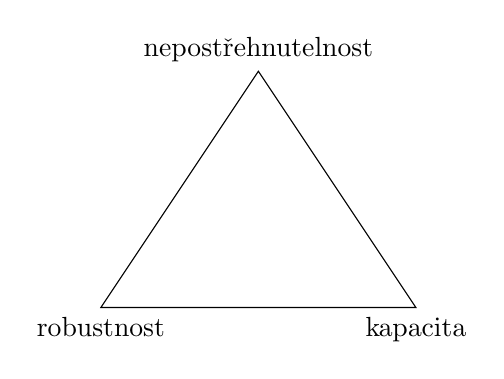
\begin{tikzpicture}
        \draw (0,0) coordinate[label=below:robustnost] --
              (4,0) coordinate[label=below:kapacita] --
              (2,3) coordinate[label=above:nepostřehnutelnost] --
              cycle;
    \end{tikzpicture}
    \caption{Trojúhelník se třemi nejvýznamnějšími vlastnostmi steganografických metod}
    \label{pic:method-property-triangle}
\end{figure}

\section{Metoda nahrazení nejméně významného bitu}
\label{sec:lsb}

\todo{popis metody LSB}

\blindtext

\blindtext

\blindtext

\section{Metoda skrývání pomocí ozvěny}
\label{sec:echo-hiding}

\todo{popis metody Echo hiding}

\blindtext

\blindtext

\subsection*{Ozvěna s~jedním semínkem na bit}
\label{sec:echo-single-kernel}

\todo{popis metody Echo single kernel}

\blindtext

\begin{figure}[hbt]
    \centering
    
\includegraphics[width=0.3\textwidth]{obrazky/placeholder.pdf}
    \caption{Ozvěna vzniklá konvolucí s~konvolučními semínky}
    \label{pic:echo-single-kernel-echo}
\end{figure}

\blindtext

\section{Metoda přímého rozprostřeného spektra}
\label{sec:dsss}

\todo{popis metody DSSS}

\blindtext

\begin{figure}[hbt]
    \centering
    
\includegraphics[width=0.3\textwidth]{obrazky/placeholder.pdf}
    \caption{Rozložení spektra pomocí metody přímého rozprostření spektra}
    \label{pic:dsss-spreading}
\end{figure}

\blindtext

\section{Metoda fázového kódování}
\label{sec:phase-coding}

\todo{popis metody fázového kódování}

\blindtext

\begin{figure}[hbt]
    \centering
    
\includegraphics[width=0.3\textwidth]{obrazky/placeholder.pdf}
    \caption{Změna fáze segmentu pro zakódování bitu}
    \label{pic:phase-coding-phase-change}
\end{figure}

\blindtext

\section{Metoda paritního kódování}
\label{sec:parity-coding}

\todo{popis metody paritního kódování}

\blindtext

\blindtext

\blindtext

\section{Metody založené na nedostatcích lidského sluchového ústrojí}
\label{sec:has}

\todo{popis metody HAS}

\blindtext

\blindtext

\blindtext

\section{Metoda využívající vlnkové transformace}
\label{sec:wavelet-transform}

\todo{popis wavelet metody}

\blindtext


\chapter{Návrh Python knihovny pro zvukovou steganografii}
\label{cha:library-design}

\todo{popis kapitoly návrh knihovny pro steganografii, důvod výběru Pythonu a NumPy}

\blindtext

\section{Struktura balíčků v~programovacím jazyce Python}
\label{sec:python-package-structure}

\todo{popis Python balíčků}

\blindtext

\blindtext

\section{Metody vybrané pro implementaci}
\label{sec:chosen-methods}

\todo{popis vybraných metod}

\blindtext

\blindtext

\section{Popis vlastní metody digitální zvukové steganografie}
\label{sec:own-method}

\todo{popis vlastní metody}

\blindtext

\blindtext


\chapter{Implementace a~testování}
\label{cha:implementation}

\todo{popis kapitoly implementace}

\blindtext

\section{Struktura modulů knihovny}
\label{sec:modules}

\todo{popis modulů knihovny}

\blindtext

\blindtext

\blindtext

\section{Způsoby vyhodnocení kvality metod}
\label{sec:method-quality}

\todo{popis způsobů vyhodnocení kvality}

\blindtext

\blindtext

\blindtext

\section{Výsledky vyhodnocení jednotlivých metod}
\label{sec:method-evaluation}

\todo{výsledky vyhodnocení kvality}

\blindtext

\blindtext

\blindtext


\chapter{Závěr}
\label{cha:conclusion}

\blindtext

\blindtext

\blindtext
